\documentclass[10pt,twocolumn]{article}

\usepackage{amssymb}
\usepackage{amsmath}
\usepackage{fullpage}
\usepackage{graphicx}
\usepackage{multicol}
\usepackage{titlesec}
\usepackage{titling}
\usepackage[font=sf, labelfont={sf,bf}, margin=1cm]{caption}

\pretitle{\begin{flushleft}\LARGE}
\posttitle{\par\end{flushleft}\vskip 0.5em}
\preauthor{\begin{flushleft}
\lineskip 0.5em%
\begin{tabular}{l}}
\postauthor{\end{tabular}\par\end{flushleft}}
\predate{\begin{flushleft}}
\postdate{\par\end{flushleft}}
\titleformat*{\section}{\large\bfseries\sffamily}
\titleformat*{\subsection}{\normalsize\bfseries\sffamily}

\usepackage{lmodern}
%\renewcommand*\familydefault{\sfdefault}
\newcommand{\lm}{\fontfamily{\sfdefault}\selectfont}
\newcommand{\mb}{\mathbf}

\usepackage{abstract}
\renewcommand{\abstractnamefont}{\bfseries\sffamily\normalsize}
%fg\renewcommand*{\abstractname}{\flushleft\textbf{}}

\title{\LARGE \bfseries \lm Control of Underactuated Vehicular Traffic}
\author{Stanislav Nikolov\\Massachusetts Institute of Technology\\July 6, 2012}
\date{}

\newenvironment{myindentpar}[1]%
 {\begin{list}{}%
         {\setlength{\leftmargin}{#1}}%
         \item[]%
 }
 {\end{list}}

\begin{document}

\twocolumn[
  \begin{@twocolumnfalse}
\maketitle
\vspace{-55pt}
\begin{myindentpar}{0.25cm}
\item 
\begin{paragraph}
\newline\noindent{\lm\bfseries Abstract:} We study a class of control policies for the single headway \cite{Bando} and multi-anticipative \cite{Lenz} optimal velocity traffic model in which only a subset of cars are actuated. We prove the stability of these control policies and characterize their regions of attraction around the uniform traffic flow fixed point.
\end{paragraph}
\end{myindentpar}
\vspace{20pt}
\end{@twocolumnfalse}
]

% Misc stuff to talk about
% Traffic can actually smooth out by itself depending on the parameter governing the dynamics. Can show this analytically for linear dynamics, and demonstrate it for nonlinear dynamics.

% describe / motivate your system
\section{Introduction}
A recent study by the U.S. Treasury Department found that traffic in the United States wasted 1.9 billion gallons of gas. Other studies have suggested that people in the United States spent as many as 5 billion hours in traffic, resulting in as much as \$100 billion in lost productivity.

Traffic jams form for a variety of reasons. Disturbances, such as traffic accidents or road bottlenecks are a familiar and obvious cause. However, traffic jams are often observed to form spontaneously without any apparent disturbance. Even if all vehicles have the same velocity and headway (distance to the car in front), this configuration is often unstable. Drivers are not perfect, and under certain conditions, small disturbances in the headways and velocities are amplified, leading to a self-sustaining traffic jam. 

With the possibility of street-legal, self-driving robotic cars joining regular cars on the road in the near future, it is interesting to consider traffic as an underactuated dynamical system, and the problem of smoothing out traffic jams as an underactuated control problem. %PLACEMENT!!!

The theory of traffic jams has attracted a broad community of researchers and a diverse set of modeling approaches, including fluid models \cite{}, cellular automata models \cite{}, and car-following models \cite{}. Here, we focus on car-following models and the vehicle dynamics that have been proposed to reproduce self-sustaining traffic jams. Bando et al. \cite{Bando} propose the optimal velocity model (OVM) and study the local linear stability about the uniform flow steady state. However, they do not study the region of attraction around the fixed point. Peng et al. \cite{Peng} present a linear traffic model in which each vehicle regulates its headway using proportional-derivative control. Despite its ease of analysis and usefulness as a tool to study linearized dynamics, the linear model alone does not prevent negative velocities or vehicle collisions, nor does it robustly generate self-sustaining traffic jams.\footnote{The system would need modes with purely imaginary eigenvalues.}

In addition to models of the passive vehicle system, many have proposed control policies to smooth out traffic jams. Konishi et al. \cite{Konishi} studied the stability of a controlled OVM. Konishi's system is {\em fully-actuated} since one has control authority over each car. As robotic cars (such as Google's self-driving car \cite{Thrun}) being to join regular cars on the road, a more realistic scenario would be one in which the system is {\em underactuated}. In an underactuated vehicle system, one can only control a subset of {\em active} cars while the rest of the cars ({\em passive} cars) follow a given dynamics. In this work, I propose a simple control policy that stabilizes an otherwise unstable system by controlling only a subset of the cars. In another fully-actuated approach to control, Lenz et al. \cite{} consider the stabilizing effect of an OV function that takes into account multiple headways. This model also admits an underactuated version. % AND YOU'VE IMPLEMENTED IT?

\section{Car Following Model}
In order to talk about stabilizing vehicular traffic, we first present an idealized model of traffic flow. We model traffic as $N$ vehicles with positions $x_n$ and velocities $v_n$ driving counterclockwise on a single-lane circular road of circumference $L$.\footnote{A ciruclar road may be thought of as an idealization of the circuit roads around many cities.} The cars are arranged such that car $i-1$ precedes car $i$. Each car has a headway (the free space in front) of $\Delta x_n$.

To model vehicle motion, we must model a driver's reaction to her vehicle's headway, and in particular, how the driver should accelerate or decelerate in response to the headway. Bando et al \cite{Bando} outline two popular reaction models --- the optimal distance model and the optimal velocity model. In the optimal distance model, the driver tries to regulate the headway to a desired value, accelerating if too far from the car in front and decelerating if too close. In the optimal velocity model, the driver tries to maintain an optimal velocity computed from the headway, accelerating when below the optimal velocity and decelerating when above it. We will consider the latter model, which has the following equations of motion:
\begin{gather}
\label{ovm1} \dot{x}_n = v_n\\
\label{ovm2} \dot{v}_n = a\left(V(\Delta x_n) - v_n\right)
\end{gather}
where $a$ is the driver sensitivity and $V$ is the optimal velocity function. A common choice for $V$ \cite{Bando} is
\begin{gather*}
V(\Delta x)=\tanh(\Delta x - 2) + \tanh(2)
\end{gather*}

% SHOW GRAPH of V and V'
\begin{figure}[!h]
\lm
\begin{center}
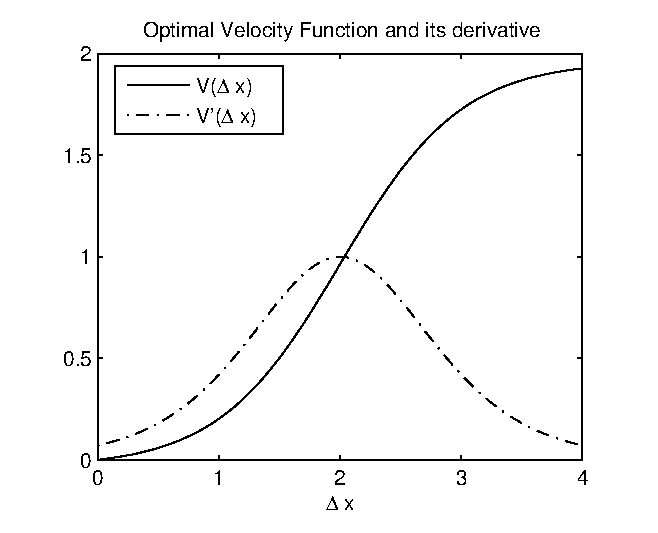
\includegraphics[width=3in]{vopt}
\end{center}
\caption{\label{fig:vopt} Optimal velocity function and its derivative.}
\end{figure}

Using this model, we can study the stability of uniform traffic flow.

\subsection{Linear Stability Analysis}
It is clear that the OVM equations of motion are satisfied when there is uniform traffic flow, i.e. when all cars have headway $L/N$ and velocity $V(L/N)$. In terms of car positions, this can be expressed as
\begin{gather}
x_n^*=bn + V(b)t
\intertext{where}
b=\frac{L}{N}
\end{gather}
This represents a fixed point in headway-velocity space. To study the stability of this fixed point, we express $x_n$ as the uniform flow steady state $x_n^*$ plus some perturbation $y_n$
\begin{gather}
x_n=x_n^*+y_n.
\end{gather}
Linearizing (\ref{ovm1}) and (\ref{ovm2}) and observing that $\dot{y}_n=\dot{x}_n$ and $\ddot{y}_n=\ddot{x}_n$ gives us the linearized equation for $y_n$
\begin{gather}
\label{ovml} \ddot{y}_n = a\left(f\Delta y_n - \dot{y}_n \right)
\intertext{where $f$ is the derivative of $V$ at the uniform flow headway $b$}
f=V'(b).
\end{gather}
We solve (\ref{ovml}) by considering as solutions the time-evolving discrete Fourier modes
\begin{gather}
y_k(n,t)=\exp\left(i\alpha_k n + zt\right)\\
\alpha_k = \frac{2\pi}{N}k (k=0,1,\dots,N-1)
\intertext{where}
z=u+iv
\intertext{and $u$ and $v$ are real.}
\end{gather}
Plugging $y_k(n,t)$ into (\ref{ovml}), we get a condition on $a,z,f$ and $\alpha_k$:
\begin{gather}
\label{zcond} z^2 + az - af\left(e^{i\alpha_k} - 1\right) = 0
\end{gather}
Each mode $e^{i\alpha_kn}$ represents a spatial wave of car positions (relative to uniform flow) and evolves in time according to $z$. The uniform flow fixed point is stable whenever each of the $N$ spatial modes decays, i.e. whenever the real part of $z$ is negative for all $k$. Let us characterize the values of $a$ and $f$ for which this is the case. Expanding (\ref{zcond}) and treating the real and imaginary parts separately, we get
\begin{gather}
\label{stbl1} u^2 + au + af(1 - \cos(\alpha_k) ) - v^2\\
\label{stbl2} 2uv + av - af\sin(\alpha_k) = 0. 
\end{gather}
Solving (\ref{stbl1}) for $u$ and requiring $u<0$ gives
\begin{gather}
u = \frac{-a \pm \sqrt{a^2 - 4(af(1-\cos(\alpha_k))-v^2)}}{2} < 0
\end{gather}
\begin{align}
 a^2 - 4(af(1-\cos(\alpha_k))-v^2) &< a^2\\
 - 4(af(1-\cos(\alpha_k))-v^2) &< 0\\
\label{stbl3}  af(1-\cos(\alpha_k)) &> v^2
\end{align}
In (\ref{stbl3}), $v$ is unknown, but solving (\ref{stbl2}) for $u$ and requiring $u<0$ will give us a bound on $v$.
\begin{gather}
u = \frac{af\sin(\alpha)-av}{2v} < 0
\end{gather}
\begin{align}
 \frac{f\sin(\alpha_k)}{v} - 1 &< 0\\
\label{stbl4}  |v| &> f\sin(\alpha_k)
\end{align}
Combining (\ref{stbl3}) and (\ref{stbl4}), we have
\begin{align}
af(1-\cos(\alpha_k)) &> f^2\sin^2(\alpha_k)\\
 f &< \frac{a(1-\cos(\alpha_k))}{\sin^2(\alpha_k)}\\
 f &< \frac{a(1-\cos(\alpha_k))}{1-\cos^2(\alpha_k)}\\
 f &< \frac{a(1-\cos(\alpha_k))}{(1+\cos(\alpha_k))(1-\cos(\alpha_k))}\\
\label{stbl5}  f &< \frac{a}{2\cos^2(\frac{\alpha_k}{2})}
\end{align}
Recalling that the uniform flow is not stable unless (\ref{stbl5}) is true for all $k$, we get a simple necessary and sufficient stability condition on $a$ and $f$:
\begin{gather}
f < \frac{a}{2}
\end{gather}

This result is summarized visually in Figure \ref{fig:stblregion}.

\begin{figure}[!h]
\lm
\begin{center}
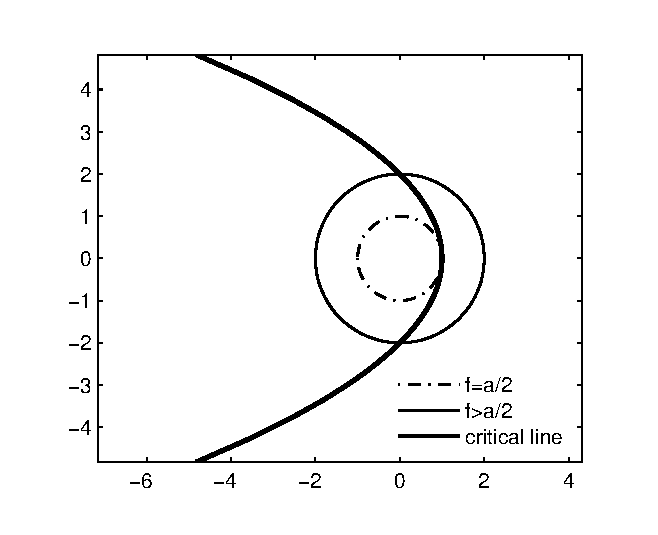
\includegraphics[width=3in]{stblregion}
\end{center}
\caption{ \label{fig:stblregion} The stability of the uniform flow fixed point is characteried by a critical line in the $(f,\alpha)$ plane in polar coordinates. Here, $\alpha$ is taken to be a continuous parameter for simplicity.}
\end{figure}

\section{Analysis of Control Policies}
Suppose that we can control a subset of the cars. In this section, we propose ???????HOW MANY, WHAT KIND, ETC????????? control policies that enlarge ????????WORDING????????? the stable region of the uniform flow.  

\subsection{Control Using Caution Functions}
Let us call the cars we can control {\em active} and the rest of the cars {\em passive}. Let $\mathcal{A}$ be the set of active car indices and $\mathcal{P}$ be the set of passive car indices. 

% TRANSITION

Consider the following control policy for active cars. Whenever an active car has headway $\Delta x$, its driver pretends that the headway is actually $c(\Delta x)$, where $c$ is nonnegative, sublinear, monotonically increasing, and differentiable on $(0,\infty)$. The car then follows the optimal velocity dynamics as usual. The modified dynamics are
\begin{align}
\dot{x}_n &=& v_n, &n=1, \dots, N\\
\dot{v}_n &=& a\left(V(\Delta x_n) - v_n \right), &n \in \mathcal{P}\\
\dot{v}_n &=& a\left(V(c(\Delta x_n)) - v_n \right), &n \in \mathcal{A}
\end{align}
or in headway-velocity space,
\begin{align}
\dot{\Delta x}_n &=& v_{n-1}-v_n, &n=1,\dots, N\\
\dot{v}_n &=& a\left(V(\Delta x_n) - v_n \right), &n \in \mathcal{P}\\
\dot{v}_n &=& a\left(V(c(\Delta x_n)) - v_n \right), &n \in \mathcal{A}
\end{align}
Let us find the fixed point of these dynamics in headway-velocity space and analyze its stability. Setting $\dot{\Delta x}_n$ and $\dot{v}_n$ to 0, we get
\begin{align}
\label{cfp1} v_{n-1} &=& v_n, &n=1, \dots, N\\
v_n &=& V(\Delta x_n), &n \in \mathcal{P}\\
v_n &=& V(c(\Delta x_n)), &n \in \mathcal{A}
\end{align}
Let us now consider two adjacent cars $p$ and $a$, with the $p$th passive and the $a$th active. Because their velocities must be equal we have 
\begin{gather}
V(\Delta x_p)=V(c(\Delta x_a)).
\intertext{For monotonic $V$, this implies}
\label{cfp2} \Delta x_p=c(\Delta x_a).
\end{gather}
Equations (\ref{cfp1}) and (\ref{cfp2}), together with the constraint that all headways must sum to $L$ determine the fixed point.



\section{Numerical Simulations}

\begin{figure}[!h]
\lm
\begin{center}
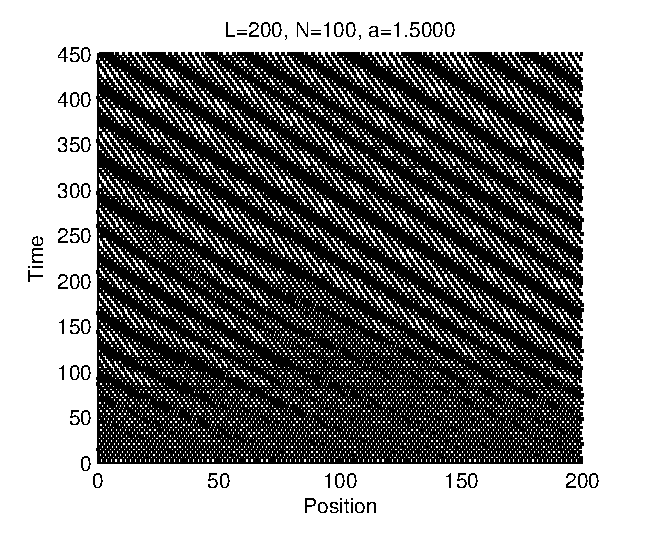
\includegraphics[width=3in]{instability}
\end{center}
\caption{ \label{fig:instability} For sensitivity $a<2f$, the uniform traffic flow configuration is unstable. Starting close to uniform flow, the system is pushed away toward a self sustaining traffic jam.}
\end{figure}


\begin{figure}[!h]
\lm
\begin{center}
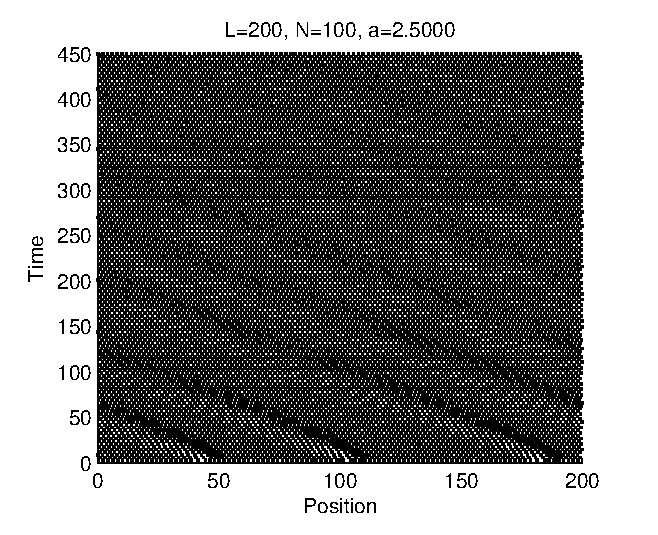
\includegraphics[width=3in]{smoothed}
\end{center}
\caption{ \label{fig:smoothed} For sensitivity $a>2f$, the uniform traffic flow configuration is stable. Starting away from uniform flow, the disturbances in the vehicle velocities and headways are smoothed out.}
\end{figure}

% describe the algorithmic approach you selected and why
\section{Algorithmic Approach}

LQR cost doesn't really handle rewarding high velocity (though it can specify an arbitrarily high desired velocity). SGD can do any objective function.

LQR doesn't know about the constraint that all inter-car distances have to sum to the circumference. Hence, we have to remove the Nth spacing and its derivatives from the state in order to manually enforce the constraint.

\section{Results}

\subsection{Circular Topology}

\paragraph{No delay} Traffic eventually smooths out by itself but it takes a very long time. Adding active cars dramatically reduces the time it takes to smooth out traffic. 

Using LQR: Because the LQR objective prescribes a desired distance between cars, and cars will naturally want to spread out evenly over the whole circle, the active cars end up picking up the ``slack'' in order to make all the distances add up to the circumference of the circle. (This is not the whole story. When the circumference is less than the total sum of the desired spacings, LQR optimizes for cars having the same velocity and takes a penalty on desired distances.)

An interesting observation is that with a small number of active cars, this act of picking up slack can make the distances in front of the active cars oscillate, leading to negative distances. As more active cars are added, each individual car is less burdened with making the distances sum to the cirucmference, and no distances ever become negative.

The passive system only stable for certain gains (how do you know which ones? Make a distinction between stability=smoothness and stability=things not blowing up. That is, self-sustaining traffic is stable in a mathematical sense, but velocities blowing up is not). However, the addition of active cars stabilizes systems that would have otherwise been unstable.

\paragraph{Delay}

Delay appears to make the system take even more time to smooth out (does it? you changed the timestep --- watch out!). However, I could not get it to do self sustaining traffic.



Linear Topology


% list any surprises / difficulties that you encountered (so that we can all learn from them)
\section{Discussion}  

The qualitative behavior of traffic models is difficult to understand. Some models seem to form shocks and rarefactions and others seem to not. It is difficult to tell whether this is due to the parameter setting or an inherent limitation in the model.

Aw Rascle model seems more aggressive. It is also nonlinear. Hence shocks?

Numerical Instability (preventing collisios but not updating velocities and accelerations to 0). Leads to NaN scores for sgd.

Need small deltas for sgd for small ks.

Need more clever penalty function, since cars can be | o o o o o o o o o           o o o | (good, but high penalty because of gap) or | o ooo o o ooo o oo o o o ooo oo  oo| (bad but good penalty becase of no gap)

How to handle infinite cost for SGD. For example, if we have a 1/avgvelocity term in the cost function and all the cars stop, the cost will be infinite. The cars will all stop in finite time if the active gains are set to zero.

Integrating the total cost over time might not be the best thing to do. What we want is the cost in the long run. Otherwise, systems that smooth out can often do far worse overall than systems that don't.

Key contribution of the approach: Control and verification of non-analytical systems.

\end{document}
